\documentclass[aspectratio=169]{beamer}
\usepackage{tikz}
\usetikzlibrary{arrows,shapes}
\tikzstyle{vertex}=[circle,fill=black!25,minimum size=10pt,inner sep=0pt]
\tikzstyle{blue vertex}=[circle,fill=blue!100,minimum size=10pt,inner sep=0pt]
\tikzstyle{red vertex}=[circle,fill=red!100,minimum size=10pt,inner sep=0pt]
%\tikzstyle{label}=[thin, draw=black, align=center,minimum width=0.5cm, minimum height=0.5cm,fill=white]
\tikzstyle{edge} = [draw,thick,-]
\tikzstyle{red edge} = [draw, line width=5pt,-,red!50]
\tikzstyle{black edge} = [draw, line width=5pt,-,black!20]
\tikzstyle{weight} = [font=\smaller]


\usepackage{amssymb,amsmath}
\usepackage{graphicx}
\usepackage{url}
\usepackage{color}
\usepackage{relsize}		% For \smaller
\usepackage{url}			% For \url
\usepackage{epstopdf}	% Included EPS files automatically converted to PDF to include with pdflatex
\usepackage{pagenote}[continuous,page]

%For MindMaps
% \usepackage{tikz}%
% \usetikzlibrary{mindmap,trees,arrows}%

%%% Color Definitions %%%%%%%%%%%%%%%%%%%%%%%%%%%%%%%%%%%%%%%%%%%%%%%%%%%%%%%%%
%\definecolor{bordercol}{RGB}{40,40,40}
%\definecolor{headercol1}{RGB}{186,215,230}
%\definecolor{headercol2}{RGB}{80,80,80}
%\definecolor{headerfontcol}{RGB}{0,0,0}
%\definecolor{boxcolor}{RGB}{186,215,230}

%%% Save space in lists. Use this after the opening of the list %%%%%%%%%%%%%%%%
%\newcommand{\compresslist}{
%	\setlength{\itemsep}{1pt}
%	\setlength{\parskip}{0pt}
%	\setlength{\parsep}{0pt}
%}

%\setbeameroption{show notes on top}

% You should run 'pdflatex' TWICE, because of TOC issues.

% Rename this file.  A common temptation for first-time slide makers
% is to name it something like ``my_talk.tex'' or
% ``john_doe_talk.tex'' or even ``discrete_math_seminar_talk.tex''.
% You really won't like any of these titles the second time you give a
% talk.  Try naming your tex file something more descriptive, like
% ``riemann_hypothesis_short_proof_talk.tex''.  Even better (in case
% you recycle 99% of a talk, but still want to change a little, and
% retain copies of each), how about
% ``riemann_hypothesis_short_proof_MIT-Colloquium.2000-01-01.tex''?

\mode<presentation>
{
  % A tip: pick a theme you like first, and THEN modify the color theme, and then add math content.
  % Warsaw is the theme selected by default in Beamer's installation sample files.

  %%%%%%%%%%%%%%%%%%%%%%%%%%%% THEME
  %\usetheme{Madrid}		% No subsection
  \usetheme{AnnArbor}  % Subsection on top, no color


  %\usetheme{Antibes}
  %\usetheme{Bergen}
  %\usetheme{Berkeley}		% bem bacana - menu esquerdo
  %\usetheme{Berlin}
  %\usetheme{Boadilla}
  %\usetheme{boxes}
  %\usetheme{CambridgeUS}		% bem bacana - menu superior
  %\usetheme{Copenhagen}
  %\usetheme{Darmstadt}
  %\usetheme{default}
  %\usetheme{Dresden}
  %\usetheme{Frankfurt}
  %\usetheme{Goettingen}
  %\usetheme{Hannover}		% bem bacana - menu esquerdo
  %\usetheme{Ilmenau}
  %\usetheme{JuanLesPins}
  %\usetheme{Luebeck}
  %\usetheme{Malmoe}
  %\usetheme{Marburg}		% bem bacana - menu direito
  %\usetheme{Montpellier}
  %\usetheme{PaloAlto}		% bem bacana - menu esquerdo
  %\usetheme{Pittsburgh}
  %\usetheme{Rochester}		%bacana
  %\usetheme{Singapore}
  %\usetheme{Szeged}
  %\usetheme{Warsaw}

  %%%%%%%%%%%%%%%%%%%%%%%%%%%% COLOR THEME
  %\usecolortheme{default}		% branco, azul clarinho
  \usecolortheme{crane}		% Very yellow (ok)

  %\usecolortheme{albatross}		% azul escuro, massa
  %\usecolortheme{beetle}		% cinza, menu azul
  %\usecolortheme{dolphin}		% azul e branco, legal
  %\usecolortheme{dove}			% cinza e branco, feio
  %\usecolortheme{fly}			% todo cinza, horrível
  %\usecolortheme{lily}			% parece o default
  %\usecolortheme{orchid}		% azul e branco, ok
  %\usecolortheme{rose}			% branco e violeta-claro, bonito
  %\usecolortheme{seagull}		% cinza, feio
  %\usecolortheme{seahorse}		% nhé, meio feio
  %\usecolortheme{sidebartab}		% Azul, branco, destaque na tab, interessante
  %\usecolortheme{structure}		% bichado
  %\usecolortheme{whale}		% Azul e branco, bem bonito

  %%%%%%%%%%%%%%%%%%%%%%%%%%%% OUTER THEME
  \useoutertheme{default}
  %\useoutertheme{infolines}
  %\useoutertheme{miniframes}
  %\useoutertheme{shadow}
  %\useoutertheme{sidebar}
  %\useoutertheme{smoothbars}
  %\useoutertheme{smoothtree}
  %\useoutertheme{split}
  %\useoutertheme{tree}

  %%%%%%%%%%%%%%%%%%%%%%%%%%%% INNER THEME
  \useinnertheme{circles}
  %\useinnertheme{default}
  %\useinnertheme{inmargin}
  %\useinnertheme{rectangles}
  %\useinnertheme{rounded}

  %%%%%%%%%%%%%%%%%%%%%%%%%%%%%%%%%%%

  \setbeamercovered{invisible} % or whatever (possibly just delete it)
  % To change behavior of \uncover from graying out to totally
  % invisible, can change \setbeamercovered to invisible instead of
  % transparent. apparently there are also 'dynamic' modes that make
  % the amount of graying depend on how long it'll take until the
  % thing is uncovered.

}


% Get rid of nav bar
\beamertemplatenavigationsymbolsempty

% Use short top
%\usepackage[headheight=12pt,footheight=12pt]{beamerthemeboxes}
%\addheadboxtemplate{\color{black}}{
%\hskip0.5cm
%\color{white}
%\insertshortauthor \ \ \ \
%\insertframenumber \ \ \ \ \ \ \
%\insertsection \ \ \ \ \ \ \ \ \ \ \ \ \ \ \ \ \  \insertsubsection
%\hskip0.5cm}
%\addheadboxtemplate{\color{black}}{
%\color{white}
%\ \ \ \
%\insertsection
%}
%\addheadboxtemplate{\color{black}}{
%\color{white}
%\ \ \ \
%\insertsubsection
%}

% Insert frame number at bottom of the page.
% \usefoottemplate{\hfil\tiny{\color{black!90}\insertframenumber}}

%% makes the ppagenote command for figure references at the end.

\usepackage[english]{babel}
%qq\usepackage[latin1]{inputenc}
\usepackage{CJKutf8}
\usepackage{subfigure}

\usepackage{times}
\usepackage[T1]{fontenc}

\makepagenote
\renewcommand{\notenumintext}[1]{}
\newcommand{\ppagenote}[1]{\pagenote[Page \insertframenumber]{#1}}

\title[Programming Challenges]{GB20602 - Programming Challenges}
\author[Claus Aranha]{Claus Aranha\\{\footnotesize caranha@cs.tsukuba.ac.jp}}
\institute[U. Tsukuba]{University of Tsukuba, Department of Computer Sciences}


\subtitle[Week 7: Strings]{Week 7 - String Problems}
\date[]{{\smaller(last updated: \today)}}

\begin{document}
\begin{CJK}{UTF8}{ipxm}

\begin{frame}
\maketitle
\vfill

\hfill Version 2022.1
\end{frame}

\section{Introduction}

\begin{frame}{Topics for this week}
  Topics for this week:
  \begin{itemize}
    \item String Matching;
    \begin{itemize}
      \item Naive search;
      \item KMP;
      \item Z-Algorithm;
    \end{itemize}
    \item Strings algorithms with DP;
    \begin{itemize}
      \item Edit Distance
      \item Common substring
      \item Palindromes
    \end{itemize}
    \item Suffix Trie
    \begin{itemize}
      \item Suffix Tree; -- idea
      \item Suffix Array; -- Implementation
    \end{itemize}
  \end{itemize}
\end{frame}

\begin{frame}{Why Study String Problems?}
    \begin{exampleblock}{}
      The manipulations of string is a common task in real life applications such as:

      \begin{itemize}
        \item Analysis of Bioinformatics Gene Data;
        \item Pre-processing/wrangling, of API data (ex: JSON)
        \item Text processing from human interfaces (natural language)
      \end{itemize}
    \end{exampleblock}

    \begin{block}{Characteristics of String Problems}
      \begin{itemize}
      \item "Parsing" of inputs with special rules;
      \item Using Dynamic Programming for finding patterns;
      \item Special data structures for storing patterns;
      \end{itemize}
    \end{block}
\end{frame}




\section{String Matching}

\begin{frame}
  \begin{center}
    {\bf Part I: String Matching}
  \end{center}
\end{frame}

\subsection{Basics}

\begin{frame}[fragile]{The String Matching Problem}
  \begin{block}{Definition}
    Given a string $T$ (also called {\bf text}), we want to test if the substring $P$ (also called {\bf pattern}) exists in $T$.
    \bigskip

    If $P$ exists in $T$, we want to know the {\bf index} of the start of $P$ in $T$.
  \end{block}\bigskip

  Example:
\begin{verbatim}
T: STEVEN EVENT

P: EVE            indexes: 2 and 7
P: EVENT          indexes: 7
P: EVENING        indexes: -1 or NULL
\end{verbatim}
\end{frame}

\begin{frame}{String Matching and Libraries}

  \begin{block}{String Matching with the standard functions}
    \begin{itemize}
      \item C/C++: strstr(T,P) or T.find(P)
      \item Python: T.find(P)
      \item Java: T.indexOf(P)
    \end{itemize}
  \end{block}

  Using the standard library is usually bug-free, but sometimes you need to code string search by hand:
  \begin{itemize}
    \item Specific Matching Function (ex: "1" == "I", "0" == "O");
    \item Match in multiple directions (graph, grind);
    \item Match multiple strings at once;
    \item etc...
  \end{itemize}\bigskip
\end{frame}

\begin{frame}[fragile]{String Matching: Complete Search}

  For every character $T_i$, test if $P$ begins at that position.\bigskip

\begin{verbatim}
for (int i = 0; i < |T|; i++)
  bool match = true;
  for (int j = 0; j < |P| && match; j++)
    if (i+j >= |T| || P[j] != T[i+j])
      match = false;
  if (match)
    printf("Match P at index %d\n", i);
\end{verbatim}

{\bf Number of Steps}:
  \begin{itemize}
    \item Average case: $O(|T|)$ -- For natural T and small P;
    \item Worst case: $O(|T|\times|P|)$;
    \begin{itemize}
      \item T = AAAAAAAAAAAAB
      \item P = AAAAAAAB
    \end{itemize}
  \end{itemize}
\end{frame}

\subsection{Knuth-Morris-Pratt}
\begin{frame}[fragile]
  \frametitle{The Knuth-Morris-Pratt (KMP) Algorithm}

  \begin{itemize}
    \item Complete Search can be very expensive if the prefix of $P$ happens many times in $T$.
    \item In 1977, Knuth, Morris and Pratt developed an algorithm that {\bf uses these prefixes} to realize fast string matching.
  \end{itemize}

  \begin{block}{Basic Idea}
    \begin{itemize}
    \item The KMP algorithm identifies "borders" in the partial match between $P$ and $T$.
    \item These borders are characterized by identical prefixes and sufixes in the T-P match.
    \item The algorithm uses these matches to advance the indexes of $T$ and $P$, greatly reducing the number of comparisons.
  \end{itemize}
  \end{block}
  The KMP algorithm is O(P+T).
\end{frame}

\begin{frame}[fragile]{KMP Algorithm -- Simulation}

{\smaller
\begin{verbatim}
              1         2         3         4         5
    012345678901234567890123456789012345678901234567890
T = I DO NOT LIKE SEVENTY SEV BUT SEVENTY SEVENTY SEVEN
P = SEVENTY SEVEN
// for i from 0 to 13, KMP works like full search

                  SEVENTY SEVEN
// Here, the collision is at i=25, j = 11, But because "SEV" is
// a "border", i stays the same and j is rewinded to 3

                                  SEVENTY SEVEN
// Here we find a match with i=43, j=13; SEVEN is a border, so j
// is rewinded to 5, and i is kept the same. The algorithm
// continues matching at i=44, j=5 ("T")

                                          SEVENTY SEVEN
// KMP finds a second match
\end{verbatim}}

\end{frame}


\begin{frame}[fragile]{KMP Algorithm -- Rewind Array}

\begin{block}{}
To avoid repeated matches, the KMP algorithm builds a {\bf rewind table} $b$ (back).

\begin{verbatim}
     0 1 2 3 4 5 6 7 8 9 0 1 2 3
P =  S E V E N T Y   S E V E N \0
b = -1 0 0 0 0 0 0 0 0 1 2 3 4 5
\end{verbatim}

Following the table $b$, we know that if we find a mismatch at $j = 11$, then we need to rewing $j$ to $b[11] = 3$ to continue matching.\bigskip

The text index $i$, on the other hand, will stay the same, and go forward by 1 if $b[j] = -1$.
    \end{block}
\end{frame}

\begin{frame}[fragile]{KMP Algorithm -- PseudoCode}

  {\smaller
  \begin{exampleblock}{}
\begin{verbatim}
char T[MAX_N], P[MAX_N];    int b[MAX_N], n, m;

void kmpPreprocess() {                         // Create the Back Array
  int i = 0, j = -1; b[0] = -1;
  while (i < m) {
     while (j >= 0 && P[i] != P[j]) j = b[j];
     i++; j++;
     b[i] = j; }}

void kmpSearch() {                             // Search the substring
  int i = 0, j = 0;
  while (i < n) {
     while (j >= 0 && T[i] != P[j]) j = b[j];
     i++; j++;
     if (j == m) {
        printf("P is found at index %d in T\n", i - j);
        j = b[j]; }}}
\end{verbatim}
  \end{exampleblock}
  }
\end{frame}

\subsection{Z algorithm}

\begin{frame}[fragile]{String Matching with the Z-Algorithm}
  Another alogirthm that performs string matcfhing in linear time is the {\bf Z algorithm}.\bigskip

  The Z algorithm first makes a {\bf Search String} $S = P + 'S' + T$.\\
  The Z algorithm next constructs a {\bf Z array} of "prefix lengths".\\
  For every index $i\in S$, $Z[i]$ is the size of the prefix of $S$ that begins in $i$.\bigskip

\begin{verbatim}
T = AASABAABAAT, P = AAB, S = P + '$' + T

... Build Z Array ...
S   = AAB$AASABAABAAT
Z[S]= X10021010310210
               ^
               String matched here. Z[i] = Len(P)
\end{verbatim}
\end{frame}

\begin{frame}[fragile]{Z-Algorithm -- Pseudocode}
  \begin{block}{}
{\smaller
\begin{verbatim}
void Zarray(string S, int Z[]) {
    int n = S.length(); int L, R, k;
    L = R = 0;             // Prefix counters
    for (int i = 1; i < n; i++) {
        if (i > R) {       // Full search of prefix
            L = R = i;
            while (R < n && S[R] == S[R-L]) R++;
            Z[i] = R-L; R--;
        } else {           // Inside prefix candidate
            k = i-L;
            if (Z[k] < R-i+1) Z[i] = Z[k]; // no extension
            else {                         // prefix extension
                L = i;
                while (R < n && S[R] == S[R-L]) R++;
                Z[i] = R-L; R--;
}   }   }   }
\end{verbatim}}
  \end{block}

{\smaller {\bf Simulation:}
\url{https://personal.utdallas.edu/~besp/demo/John2010/z-algorithm.htm}}

\end{frame}

\begin{frame}{Z algorithm or KMP algorithm?}
  Should you use the Z algorithm or the KMP algorithm?\bigskip

  \begin{itemize}
    \item Both algorithms have the same time complexity: $O(T+P)$\bigskip

    \item Which algorithm is easier to understand?
    \begin{itemize}
      \item KMP calculates a recursive suffix state machine for P;
      \item Z-algorithm calculates a substring size array for T;
    \end{itemize}\bigskip
  \end{itemize}
\end{frame}



\section{String Algorithms with DP} % (6.5)

\begin{frame}
  \begin{center}
    {\bf Part II: Strings and DP}
  \end{center}
\end{frame}

\begin{frame}{String Algorithms with Dynamic Programming}
  \begin{block}{}
    Some string problems can be described as a {\bf search problem}. In this section, we will introduce two string tasks that can be solved with DP algorithms:\bigskip

    \begin{itemize}
    \item String Alignment/Edit Distance
    \item Longest Common Subsequence
    \end{itemize}
  \end{block}
  \bigskip

  It is interesting to note that substring matching is also a search problem, and that KMP / Z-algorithms can be seen as a kind of memoization.
\end{frame}

\subsection{String Alignment}
\begin{frame}[fragile]{String DP: String Alignment}

The {\bf String Alignment}\footnote{Also called Edit Distance or Levenhstein Distance, used by spellchecking algorithms!} problem is defined as follows. Align two strings, A and B, with the maximum "alignment score":\bigskip

\begin{itemize}
  \item Character A[i] and B[i] match: do nothing, score +2
  \item Character A[i] and B[i] mismatch: replace A[i], score -1
  \item Insert a space in A[i]: score -1 (equals to delete B[i])
  \item Insert a space in B[i]: score -1 (equals to delete A[i])
\end{itemize}

\begin{verbatim}
   Original    non-optimal    optimal
A: ACAATCC   | A_CAATCC     | A_CAATCC
B: AGCATGC   | AGCATGC_     | AGCA_TGC
score:       | 2-22--2- = 4 | 2-22-2-2 = 7
\end{verbatim}\bigskip
\end{frame}


\begin{frame}[fragile]{String Alignment: Bottom Up DP}

  The {\bf Complete Search} approach requires recursively testing each of the three options for each A[i] (Total cost: $O(3^n)$).\bigskip

  We can solve this in $O(n^2)$ using DP:

  \begin{itemize}
    \item $V(i,j)$: optimal score for prefix $A[1..i],B[1..j]$
    \item Start condition:
    \begin{itemize}
      \item $V(0,0) = 0$ \hspace{1cm} (Do nothing)
      \item $V(i,0) = -1\times i$, $V(0,j) = -1\times j$ \hfill (delete A or B)
    \end{itemize}
    \item Recurrence: $V(i,j) = \text{max}(C_1, C_2, C_3)$, where
    \begin{itemize}
      \item $C_1 = V(i-1, j-1) + \text{score}(A[i],B[j])$ \hfill score of match or mismatch;
      \item $C_2 = V(i-1,j) + \text{score}(A[i],\_)$ \hfill delete $A[i]$;
      \item $C_3 = V(i,j-1) + \text{score}(\_,B[j])$ \hfill delete $B[j]$;
    \end{itemize}
  \end{itemize}
\end{frame}


\begin{frame}[fragile]{String Alignment: Bottom Up DP}{Simulation Matching AGCATGC and ACAATCC}

\begin{itemize}
  \item Recurrence: $V(i,j) = \text{max}(C_1, C_2, C_3)$, where
  \begin{itemize}
    \item $C_1 = V(i-1, j-1) + \text{score}(A[i],B[j])$ \hfill score of match or mismatch;
    \item $C_2 = V(i-1,j) + \text{score}(A[i],\_)$ \hfill delete $A[i]$;
    \item $C_3 = V(i,j-1) + \text{score}(\_,B[j])$ \hfill delete $B[j]$;
  \end{itemize}
\end{itemize}

\begin{verbatim}
   |  _ |  A |  G |  C |  A |  T |  G |  C |
 _ |  0 | -1 | -2 | -3 | -4 | -5 | -6 | -7 |
 A | -1 |
 C | -2 |
 A | -3 |
 A | -4 |
 T | -5 |
 C | -6 |
 C | -7 |
\end{verbatim}

\end{frame}


\subsection{Longest Common Subsequence in String}

\begin{frame}[fragile]
  \frametitle{Problem 2: Longest Common Subsequence in Strings}
    \begin{block}{Problem Definition}
      Given strings $A$ and $B$, what is their longest common subsequence?\medskip

\begin{verbatim}
A  :   'ACAATCC'     - A_CAAT_CC
B  :   'AGCATGC'     - AGCA_TGC_
LCS:    AC AT C      - A_CA_T_C_ : ACATC
\end{verbatim}
    \end{block}\bigskip

  \begin{itemize}
    \item We can solve LCS using a modification of String Aligment;
    \item Use String Alignment DP, with different scores:
    \begin{itemize}
      \item Cost of Mismatch: $-\infty$
      \item Cost of insert/deletion: $0$
      \item Cost of Matching: $1$
    \end{itemize}
  \end{itemize}
\end{frame}

\begin{frame}
  \frametitle{Problem 3: Longest Palindrome}
    \begin{block}{Problem Description}
      A {\bf palindrome} is a string $S$ where $S = \text{rev}(S)$. For example: MADAM.\bigskip

      Given a string $T$, what is the {\bf longest palindrome} that you can create by deleting characters from $T$?
    \end{block}

    Examples:
    \begin{itemize}
    \item ADA\alert{\bf M} -- ADA
    \item MADAM -- MADAM
    \item NEVERODDOREVEN\alert{\bf ING} -- NEVERODDOREVEN
    \item RACE\alert{\bf F1}CAR\alert{\bf FAST} -- RACECAR
    \end{itemize}\bigskip

    {\bf QUIZ:} Can you solve with Full Search? String Alignment DP? Others?
  \end{frame}

\begin{frame}
  \frametitle{Longest Palindrome}
    \begin{block}{Problem Description}
      Given a string $S$ of size up to $N = 1000$ characters, what is the
      longest palindrome that you can make by deleting characters from $S$?
    \end{block}

    DP Solution:
    \begin{itemize}
    \item State Table:
      {\smaller
      \begin{itemize}
      \item len(i,j) - The largest palindrome found between $i$ and $j$
      \end{itemize}}
    \item Start Conditions:
      {\smaller
      \begin{itemize}
        \item If $l=r$ then len$(l,r)=1$.
        \item If $r=l+1 \text{ and } S[l]=S[r]$, len$(l,r)=2$, else len$(l,r)=1$.
      \end{itemize}}
    \item Transition:
      {\smaller
      \begin{itemize}
        \item If $S[l]=S[r]$, then len$(l,r)=2+\text{len}(l+1,r-1)$;
        \item else $\text{len}(l,r) = \text{max}(\text{len}(l+1,r),\text{len}(l,r-1))$
      \end{itemize}}
    \end{itemize}

    This DP has complexity $O(n^2)$
\end{frame}

\begin{frame}[fragile]
  \frametitle{Longest Palindrome}

  Longest Palindrome DP: Diagonal Table Top Down

  {\smaller
\begin{verbatim}

       len(l,r)               len(l,r)         transition:
      final state           initial state   - If A[l] == A[r]: len(diag)+2
                                            - If A[1] != A[r]: max(left,down)
  R A C E F 1 C A R     R A C E F 1 C A R

R 1 1 1 1 1 1 3 5 7   R 1 1
A   1 1 1 1 1 3 5 5   A   1 1
C     1 1 1 1 3 3 3   C     1 1
E       1 1 1 1 1 1   E       1 1
F         1 1 1 1 1   F         1 1
1           1 1 1 1   1           1 1
C             1 1 1   C             1 1
A               1 1   A               1 1
R                 1   R                 1

\end{verbatim}

  }
\end{frame}


\section{Suffix Trie/Array} % (6.6)

\begin{frame}
  \begin{center}
    {\bf Part III: Suffix Tree, Array}
  \end{center}
\end{frame}


\subsection{Outline}
\begin{frame}
  \frametitle{Suffix Trie: Definition}

  {\smaller
    \begin{block}{}
      Data structure used to find matching suffixes of multiple strings.
    \end{block}

    \vfill

    \begin{center}
    \structure{Suffix Trie for \{'CAR','CAT','RAT'\}}
    \end{center}

    \vfill

    \begin{columns}[T]
      \column{0.25\textwidth}
      All Suffixes
      \begin{enumerate}
      \item CAR
      \item AR
      \item R
      \item CAT
      \item T
      \item RAT
      \item AT
      \item T
      \end{enumerate}
      \column{0.25\textwidth}
      Sorted, Unique Suffixes
      \begin{enumerate}
      \item AR
      \item AT
      \item CAR
      \item CAT
      \item R
      \item RAT
      \item T (x2)
      \end{enumerate}
      \column{0.45\textwidth}
      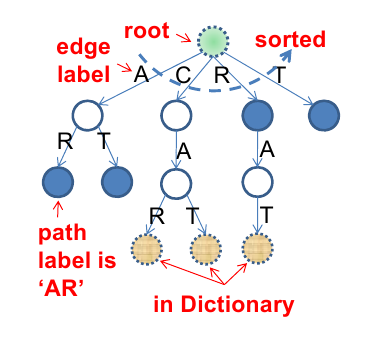
\includegraphics[width=.9\textwidth]{../img/suffixtrie_halim}\\
      % TODO: Replace suffix trie image with one of my own design
    \end{columns}
  }
\end{frame}

\begin{frame}
  \frametitle{Suffix Trie: Counting the number of substrings of GATAGACA}
  \begin{columns}[T]
    \column{0.5\textwidth}
    {\smaller
    Create all $n$ suffixes:

    \begin{tabular}{c|l}
      i & suffix\\
      \hline
      0 & GATAGACA\$\\
      1 & ATAGACA\$\\
      2 & TAGACA\$\\
      3 & AGACA\$\\
      4 & GACA\$\\
      5 & ACA\$\\
      6 & CA\$\\
      7 & A\$\\
      8 & \$\\
    \end{tabular}\bigskip

    Number of repeats of substring $m$:
    \begin{itemize}
    \item 'A': 4 subtrees
    \item 'GA': 2 subtrees
    \item 'AA': 0 subtrees
    \end{itemize}}
    \column{0.5\textwidth}
    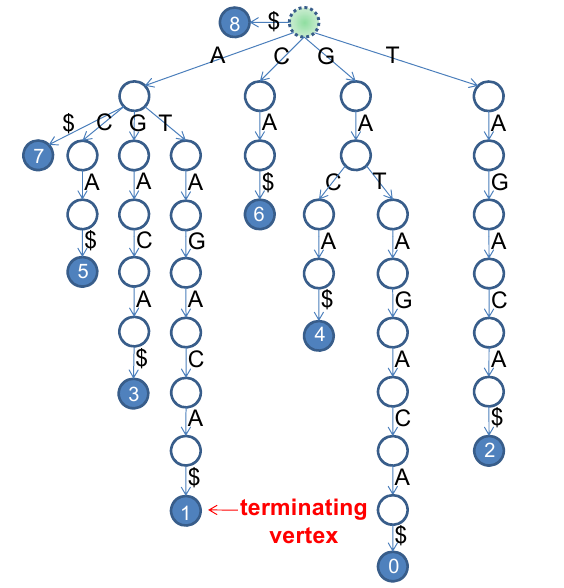
\includegraphics[width=.85\textwidth]{../img/suffixtrie_halim2}
  \end{columns}
\end{frame}

\begin{frame}
  \frametitle{Suffix Trie: Counting the number of substrings of GATACA}
  \begin{columns}[T]
    \column{0.5\textwidth}

    {\smaller

    You can make the Suffix Tree better by merging the nodes that have a single child.\bigskip

    This data structure is useful for many algorithms.\bigskip

    \begin{tabular}{c|l}
      i & suffix\\
      \hline
      0 & GATAGACA\$\\
      1 & ATAGACA\$\\
      2 & TAGACA\$\\
      3 & AGACA\$\\
      4 & GACA\$\\
      5 & ACA\$\\
      6 & CA\$\\
      7 & A\$\\
      8 & \$\\
    \end{tabular}
    }

    \column{0.5\textwidth}
    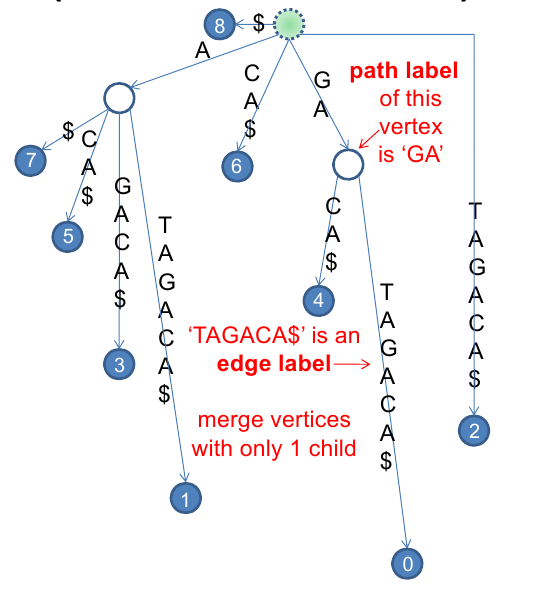
\includegraphics[width=.8\textwidth]{../img/suffixtree_halim}
    \ppagenote{Suffix Tree/Array images from Steven Halim, "Competitive Programming 3", chapter 6.6}
  \end{columns}
\end{frame}

\subsection{Uses of a Suffix Tree}
\begin{frame}
  \frametitle{Uses of a Suffix Tree 1: String Matching} {\smaller

    \structure{Assuming that we have the Suffix Tree already built},
    we can find all occurrences of substring $m$ in $T$ in time
    $O(m+\text{occ})$, where occ is the number of occurrences.

  \begin{center}
    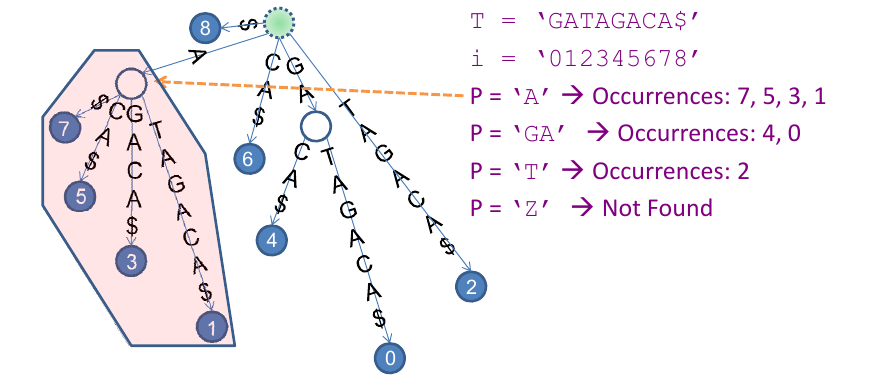
\includegraphics[width=0.9\textwidth]{../img/stringmatching_halim}
  \end{center}
  }
\end{frame}

\begin{frame}
  \frametitle{Uses of a Suffix Tree 2: Longest Repeated Substring}
  \begin{itemize}
  \item The LRS is the longest substring with number of occurrences $> 2$;
  \item The LRS is the deepest {\bf internal node} in the tree;
  \end{itemize}

  \begin{center}
    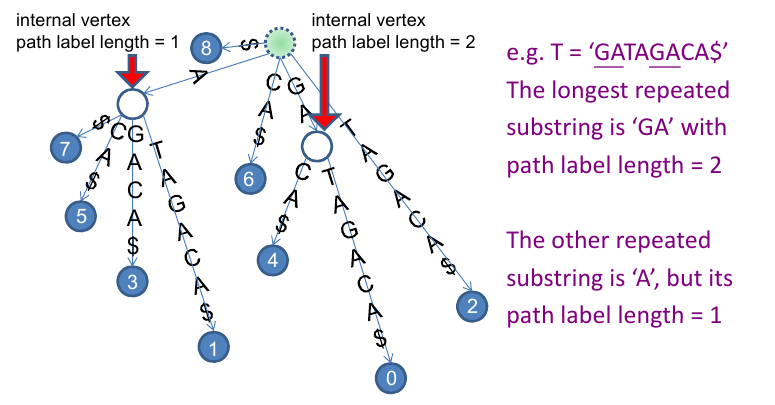
\includegraphics[width=0.75\textwidth]{../img/longestrepeatingsubstring_halim}
  \end{center}
\end{frame}

\begin{frame}
  \frametitle{Uses of a Suffix Tree 3: Longest Common Substring}
    \begin{itemize}
    \item Make a Suffix Tree of $M$ and $N$ combined, with a different ending character to each.
    \item The LCS is the deepest {\bf internal node} that includes both ending characters.
    \end{itemize}
  \begin{center}
    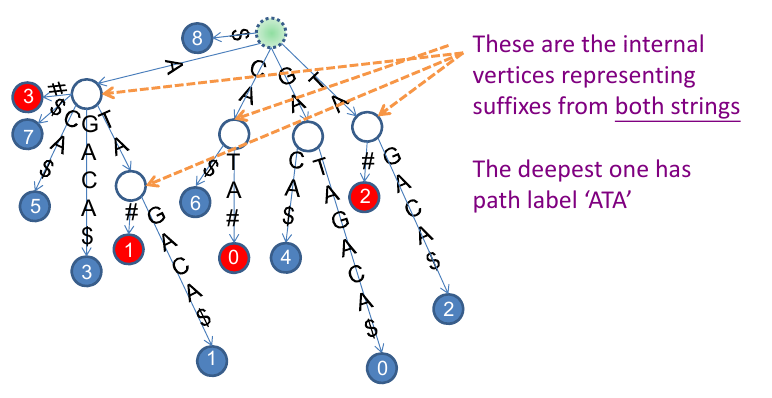
\includegraphics[width=0.75\textwidth]{../img/longestcommonsubstring_halim}
  \end{center}
\end{frame}

\subsection{Suffix Array}
\begin{frame}
  \frametitle{Suffix Array}
  \begin{itemize}
    \item The algorithms in previous slides are very efficient...\\
      ... \structure{if you have the suffix tree}

      \medskip

    \item The suffix tree can be built in $O(n)$...\\
      ... but implementation is rather complex;

      \medskip

    \item In this course, we will see the \structure{Suffix Array};

      \medskip

    \item The Suffix Array is built in $O(n\log{n})$...\\
      ... but the implementation is very simple!
  \end{itemize}

  \vfill

  \begin{block}{}
    I encourage you to study the implementation of the suffix tree by yourself!
  \end{block}
\end{frame}

\begin{frame}
  \frametitle{Suffix Array Implementation Idea}

    \begin{itemize}
    \item To make a Suffix array, make an array of all possible
      suffixes of $T$, and sort it;
    \item The order of the suffix array is the
      \structure{visit in preorder} of the suffix tree;
      % TODO: Japanese for pre-order visit
    \item We can adapt all algorithms accordingly;
    \end{itemize}

  \begin{columns}
    \column{0.4\textwidth}
    \begin{tabular}{c|l}
      i & suffix\\
      \hline
      0 & GATAGACA\$\\
      1 & ATAGACA\$\\
      2 & TAGACA\$\\
      3 & AGACA\$\\
      4 & GACA\$\\
      5 & ACA\$\\
      6 & CA\$\\
      7 & A\$\\
      8 & \$\\
    \end{tabular}
    \column{0.2\textwidth}
    Sort $\rightarrow$
    \column{0.4\textwidth}
    \begin{tabular}{c|c|l}
      i & SA[i] & suffix \\
      \hline
      0 & 8 & \$\\
      1 & 7 & A\$\\
      2 & 5 & ACA\$\\
      3 & 3 & AGACA\$\\
      4 & 1 & ATAGACA\$\\
      5 & 6 & CA\$\\
      6 & 4 & GACA\$\\
      7 & 0 & GATAGACA\$\\
      8 & 2 & TAGACA\$\\
    \end{tabular}
  \end{columns}
\end{frame}

\begin{frame}[fragile]
  \frametitle{Suffix Array: Slow Implementation}
  {\smaller
    \begin{exampleblock}{Simple Implementation}
\begin{verbatim}
#include <algorithm>
#include <cstdio>
#include <cstring>
using namespace std;
char T[MAX_N]; int SA[MAX_N],i,n;

bool cmp(int a, int b) { return strcmp(T+a, T+b) < 0; }
// O(n)

int main() {
  n = (int) strlen (gets(T));
  for (int i = 0; i < n; i++) SA[i] = i;
  sort (SA, SA+n, cmp); // O(n^2 log n) }
\end{verbatim}
\end{exampleblock}}

    This implementation is too slow for strings bigger than 1000 characters.
\end{frame}

\begin{frame}[fragile]
  \frametitle{Suffix Array: Better Implementation (1)}
  {\smaller
    \begin{exampleblock}{O(n log n) implementation using ``ranking pairs/radix sort''}
\begin{verbatim}
char T[MAX_N]; int n; int c[MAX_N];
int RA[MAX_N], tempRA[MAX_N], SA[MAX_N], tempSA[MAX_N];

void countingSort(int k) {
  int i, sum, maxi = max(300,n);                        //255 ASCII chars or n
  memset(c, 0, sizeof(c));
  for (i = 0; i < n; i++) c[i+k<n? RA[i+k] : 0]++
  for (i = sum = 0; i < maxi; i++)
    { int t = c[i]; c[i] = sum; sum += t; }             //frequency
  for (i = 0; i < n; i++)
    tempSA[c[SA[i]+k < n ? RA[SA[i]+k] : 0]++] = SA[i];
  for (i = 0; i < n; i++)                               // update suffix array
    SA[i] = tempSA[i];
}

// ... continues next slide
\end{verbatim}
    \end{exampleblock}
  }
\end{frame}

\begin{frame}[fragile]
  \frametitle{Suffix Array: Better Implementation (2)}
  {\smaller
    \begin{exampleblock}{O(n log n) implementation using ``ranking pairs/radix sort''}
\begin{verbatim}
// ... continued from last slide
void constructSuffixArray() {
  int i, k, r;
  for (i = 0; i < n; i++) { RA[i] = T[i]; SA[i] = i;}
  for (k = 1; k < n; k <<=1) {
    countingSort(k); countingSort(0); tempRA[SA[0]] = r = 0;
    for (i = 1; i < n; i++)
      tempRA[SA[i]] =
          (RA[SA[i]] == RA[SA[i-1]] && RA[SA[i]+k] == RA[SA[i-1]+k]) ?
           r : ++r;
    for (i = 0; i < n; i++)
      RA[i] = tempRA[i];
    if (RA[SA[n-1]] == n-1) break;
  }
}
\end{verbatim}
    \end{exampleblock}
  }
\end{frame}

\begin{frame}
  \frametitle{Using Suffix Array for String Matching:}
  {\smaller
    \begin{block}{}
      \begin{itemize}
      \item Do binary search two times: One to find the lower bound, one to find the upper bound;
      \end{itemize}
    \end{block}
    \begin{center}
      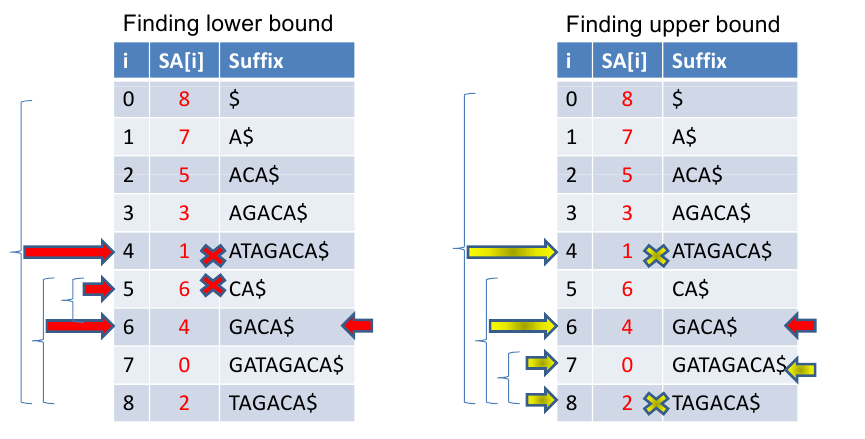
\includegraphics[width=0.8\textwidth]{../img/suffixarray_halim}
    \end{center}
  }
\end{frame}

\begin{frame}{Using Suffix Array for Longest Repeated Substring}
  {Find the pair of indexes $i$ and $i+i$ with longest common prefix.}

    \begin{center}
      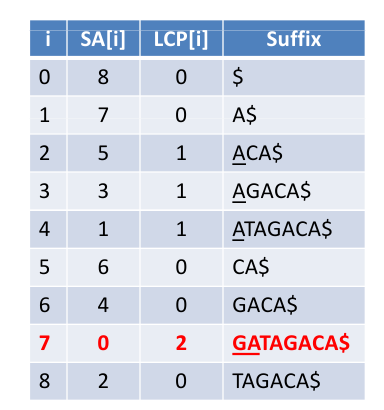
\includegraphics[width=0.4\textwidth]{../img/suffixarray2_halim}
    \end{center}
\end{frame}

\begin{frame}{Using Suffix Array for Longest Common Substring}
  {Append strings $M$ and $N$ with different endings, and find LCS}
    \begin{center}
      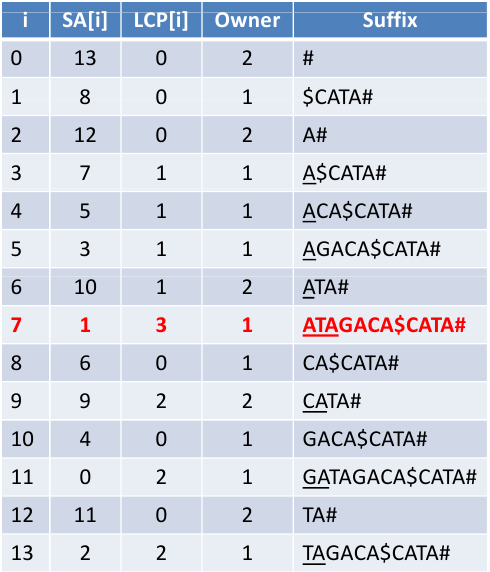
\includegraphics[width=0.36\textwidth]{../img/suffixarray3_halim}
    \end{center}
\end{frame}



%%%%%%%%%%%%%%%%%%%%%%%%%%%%%%%%%%%%%%%%%%%%%%%%%%%%
\section{Backmatter}
\begin{frame}{About these Slides}
  These slides were made by Claus Aranha, 2020. You are welcome to copy, re-use and modify this material.
  \bigskip

  Individual images in some slides might have been made by other
  authors. Please see the references in each slide for those cases.
\end{frame}

\begin{frame}[allowframebreaks]{Image Credits}
  \printnotes
\end{frame}

\end{CJK}
\end{document}
